\documentclass{article}
\usepackage{graphicx}
\title{Whale and Dolphin Identification}
\author{Matthew Harding}
\date{April 2024}

\begin{document}
\maketitle

\section{Introduction}
This project explores the problem of classifiying images of dolphin and whales to identify indivduals. This work 
is based on the \emph{Happywhale - Whale and Dolphin Identification} Kaggle competition.\par

Data for this competition contains images of over 15,000 unique individual marine mammals from 30 different species collected from 28 different research organizations. 
Individuals have been manually identified and given an individual\_id by marine researches.\par

Unlike a typical classification problem in which there is a fixed set of classes which examples of all classes within the training data, this problem required the ability to classify individuals not contained within the training dataset.

\section{Training Data}

\begin{figure}[h!]
    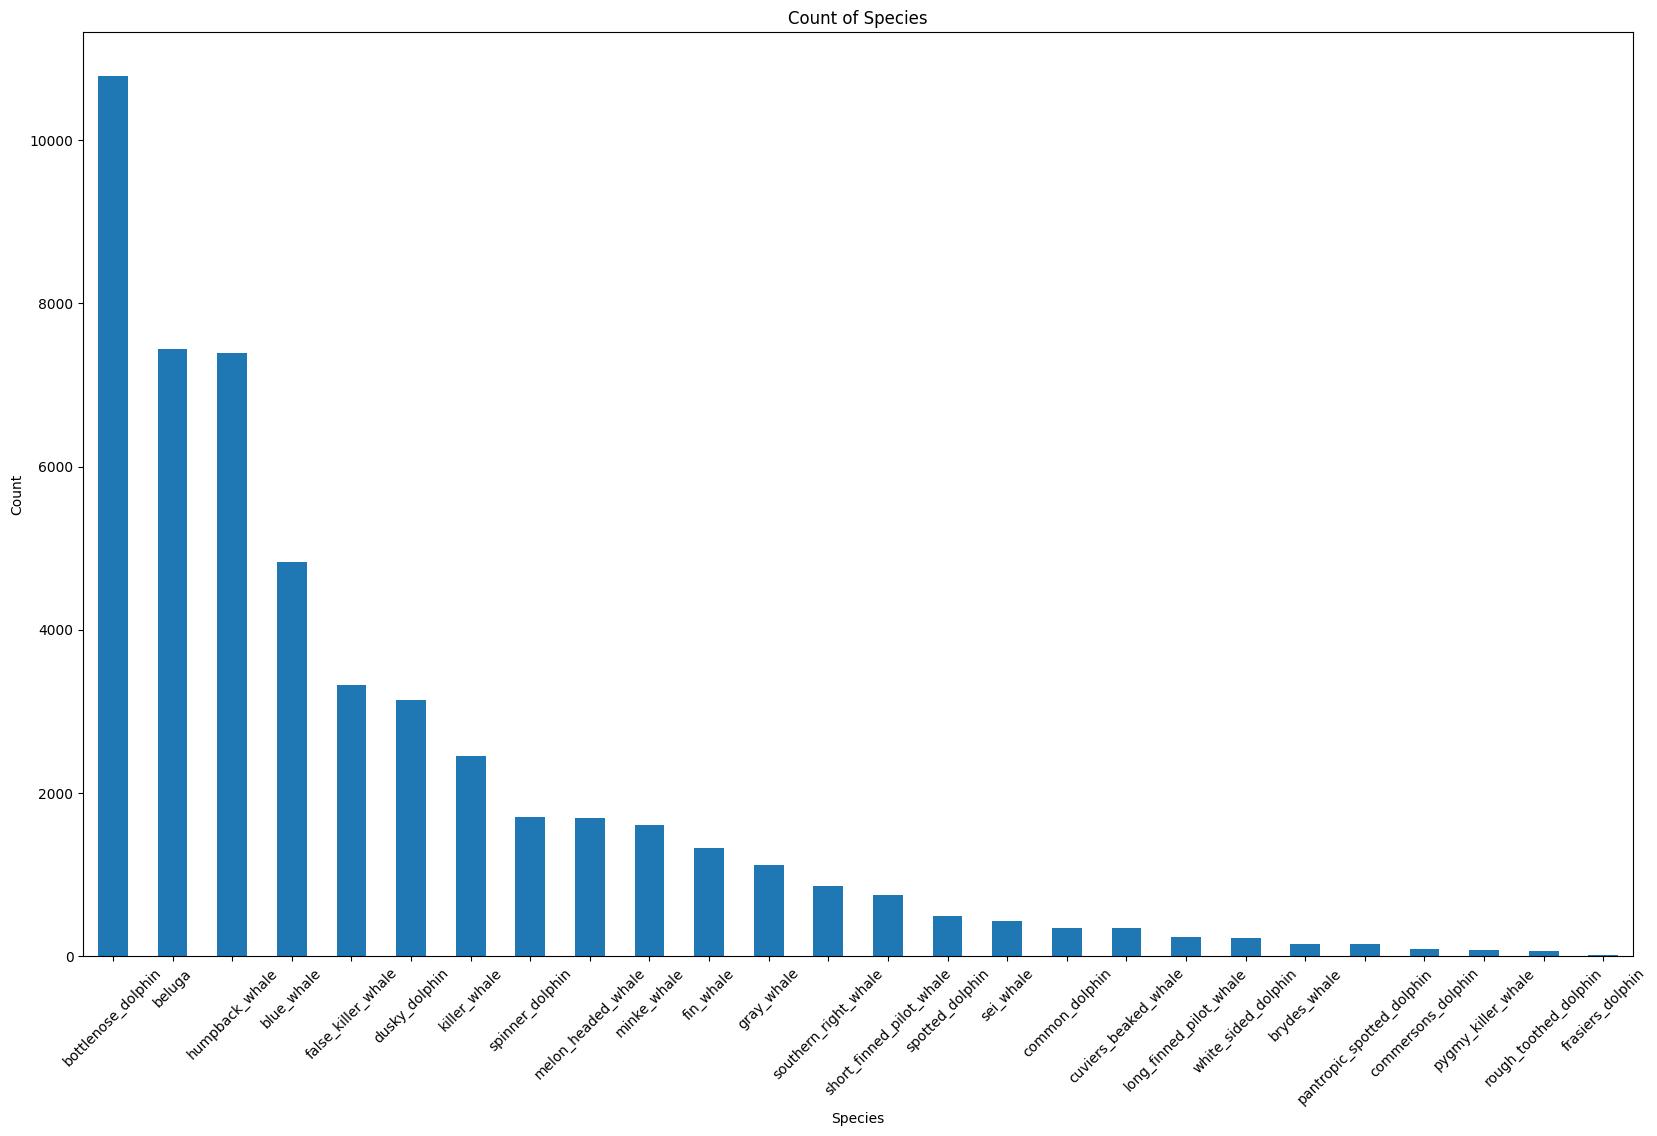
\includegraphics[width=\linewidth]{species_histogram.png}
    \caption{Number of training images per species}
    \label{fig:species_count_histogram}
\end{figure}

\begin{figure}[h!]
    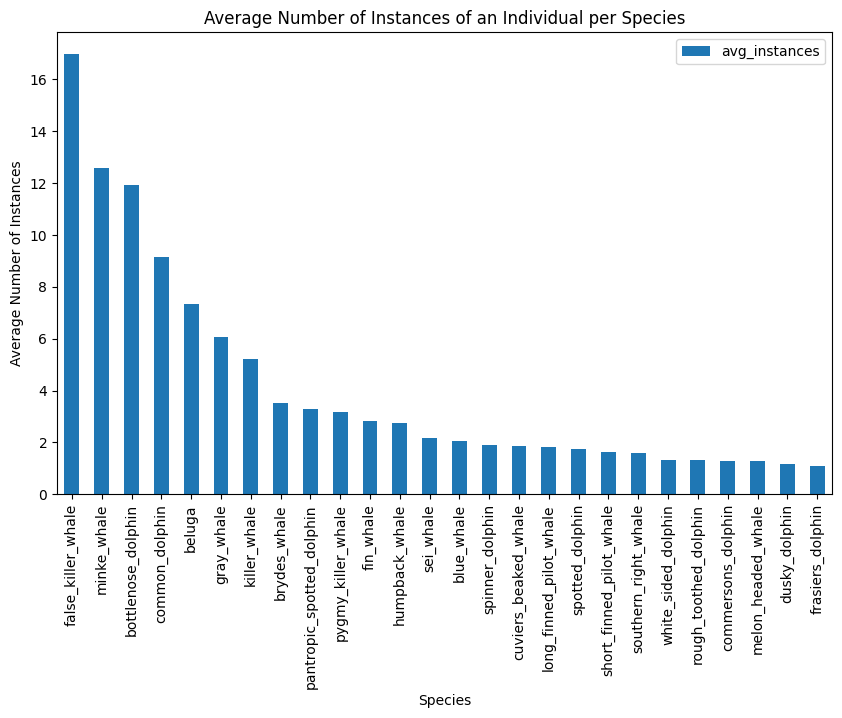
\includegraphics[width=\linewidth]{mean_individuals_histogram.png}
    \caption{Mean count of images per individual by species}
    \label{fig:individual_mean_count_histogram}
\end{figure}

Within the training data there are 51,033 labelled images. Looking at the histogram of species Figure \ref{fig:species_count_histogram}, there is a clear inbalance in the number of iamges per species with the vast majority
of labelled images being for bottlenose dolphins, beluga whales, humpback whales and blue whales. For some species the number of examples it so low it will be difficult to gain a high level of accuracy within classification.

Look at Figure \ref{fig:individual_mean_count_histogram}, the mean count of images per indivdual by species we see another imbalance with some species on average containing a large number of images per indivudal whilst others only contain one or two images per individual.


\section{Naive Classifer}

The first approach taken was to classify images

\end{document}